\documentclass[11pt]{article}
\usepackage{graphicx}
\usepackage[bookmarks=true]{hyperref}
\usepackage{bookmark}
\usepackage{hyperref}
\usepackage{csquotes}
\usepackage{float}
\usepackage{wrapfig}
\usepackage{array}
\newcolumntype{L}[1]{>{\raggedright\let\newline\\\arraybackslash\hspace{0pt}}m{#1}}
\newcolumntype{C}[1]{>{\centering\let\newline\\\arraybackslash\hspace{0pt}}m{#1}}
\newcolumntype{R}[1]{>{\raggedleft\let\newline\\\arraybackslash\hspace{0pt}}m{#1}}

\setlength{\parindent}{0pt}

\begin{document}
\begin{titlepage}
\begin{flushright}


\includegraphics[width=380px]{../global/University_of_Pretoria_Logo.png}
\newline
\newline

\textbf {\LARGE Plan for Software Aspects of Certification} \newline

\textbf {\Large (PSAC)} \newline

\centering
\includegraphics[width=100px]{../global/Logo.jpg}

\textbf {\Large Linphone for Android Group Chat (Waterfall)}\newline

\flushright \textbf {\large Version: 1.2}\newline

\centering \textbf {\large Authors:}

\begin{table}[H]
\large
\centering
\begin{tabular}{rl}
	Izak Blom & 13126777 \\
	David Breetzke & 12056503 \\
	Paul Engelke & 13093500 \\
	Prenolan Govender & 13102380 \\
	Jessica Lessev & 13049136 \\
\end{tabular}
\end{table}

Date: \today

\end{flushright}
\end{titlepage}

\setcounter{tocdepth}{3}
\setcounter{secnumdepth}{5}
\tableofcontents
\newpage
\section{Revision History}
\begin{table}[h]
\begin{tabular}{llll}
\textbf{Date}          & \textbf{Description}  & \textbf{Author}       & \textbf{Comments}   \\ \hline
\multicolumn{1}{|R{2cm}|}{23/06/2015} & \multicolumn{1}{L{4.5cm}|}{Document Creation} & \multicolumn{1}{l|}{Team Eclectic} & \multicolumn{1}{L{4cm}|}{Version 1} \\ \hline
\multicolumn{1}{|R{2cm}|}{16/08/2015} & \multicolumn{1}{L{4.5cm}|}{Grammar Correction} & \multicolumn{1}{l|}{Team Eclectic} & \multicolumn{1}{L{4cm}|}{Version 1.01} \\ \hline
\multicolumn{1}{|R{2cm}|}{28/08/2015} & \multicolumn{1}{L{4.5cm}|}{Revision 1} & \multicolumn{1}{l|}{Team Eclectic} & \multicolumn{1}{L{4cm}|}{Version 2.0} \\ \hline
\multicolumn{1}{|l|}{} & \multicolumn{1}{l|}{} & \multicolumn{1}{l|}{} & \multicolumn{1}{l|}{} \\ \hline
\multicolumn{1}{|l|}{} & \multicolumn{1}{l|}{} & \multicolumn{1}{l|}{} & \multicolumn{1}{l|}{} \\ \hline
\multicolumn{1}{|l|}{} & \multicolumn{1}{l|}{} & \multicolumn{1}{l|}{} & \multicolumn{1}{l|}{} \\ \hline
\multicolumn{1}{|l|}{} & \multicolumn{1}{l|}{} & \multicolumn{1}{l|}{} & \multicolumn{1}{l|}{} \\ \hline
\multicolumn{1}{|l|}{} & \multicolumn{1}{l|}{} & \multicolumn{1}{l|}{} & \multicolumn{1}{l|}{} \\ \hline
\multicolumn{1}{|l|}{} & \multicolumn{1}{l|}{} & \multicolumn{1}{l|}{} & \multicolumn{1}{l|}{} \\ \hline
\multicolumn{1}{|l|}{} & \multicolumn{1}{l|}{} & \multicolumn{1}{l|}{} & \multicolumn{1}{l|}{} \\ \hline
\multicolumn{1}{|l|}{} & \multicolumn{1}{l|}{} & \multicolumn{1}{l|}{} & \multicolumn{1}{l|}{} \\ \hline
\multicolumn{1}{|l|}{} & \multicolumn{1}{l|}{} & \multicolumn{1}{l|}{} & \multicolumn{1}{l|}{} \\ \hline
\multicolumn{1}{|l|}{} & \multicolumn{1}{l|}{} & \multicolumn{1}{l|}{} & \multicolumn{1}{l|}{} \\ \hline
\multicolumn{1}{|l|}{} & \multicolumn{1}{l|}{} & \multicolumn{1}{l|}{} & \multicolumn{1}{l|}{} \\ \hline
\multicolumn{1}{|l|}{} & \multicolumn{1}{l|}{} & \multicolumn{1}{l|}{} & \multicolumn{1}{l|}{} \\ \hline
\end{tabular}
\end{table}

\section{Document Approval}
\begin{table}[h]
\begin{tabular}{llll}
\textbf{Signature}     & \textbf{Printed Name} & \textbf{Title}        & \textbf{Comments}     \\ \hline
\multicolumn{1}{|l|}{} & \multicolumn{1}{L{3.5cm}|}{} & \multicolumn{1}{L{3.5cm}|}{} & \multicolumn{1}{L{4cm}|}{} \\ \hline
\multicolumn{1}{|l|}{} & \multicolumn{1}{l|}{} & \multicolumn{1}{l|}{} & \multicolumn{1}{l|}{} \\ \hline
\multicolumn{1}{|l|}{} & \multicolumn{1}{l|}{} & \multicolumn{1}{l|}{} & \multicolumn{1}{l|}{} \\ \hline
\multicolumn{1}{|l|}{} & \multicolumn{1}{l|}{} & \multicolumn{1}{l|}{} & \multicolumn{1}{l|}{} \\ \hline
\end{tabular}
\end{table}

\newpage
\section{Introduction}
Linphone is the leading open source implementation of Voice over IP (VoIP) and Instant messaging functionalities, and is compatible with iOS, Android, Blackberry, Windows Phone, Windows desktop and web browser clients. This user manual will be focused specifically on the Android aspect. 
\section{Systems Overview}

\section{Systems Configuration}
Linphone has inside a separation between the user interfaces and the core engine, allowing to create various kinds of user interface on top of the same functionalities.\\

The user interface frontends:
\begin{itemize}
\item Gtk+ interface for windows, mac and linux
\item The console interface (linphonec, linphonecsh)
\item The iPhone application built in objective C
\item The Android application running in java
\item The Windows Phone application written in C\#
\end{itemize}
Liblinphone, the core engine: this is the library that implements all the functionalities of Linphone. \\
Liblinphone is a powerful SIP VoIP video SDK that anyone can use to add audio or video call capabilities to an application. It provides a high level api to initiate, receive, terminate audio and video calls.\\
Liblinphone relies on the following software components:
\begin{itemize}
\item Mediastreamer2, a powerful multimedia SDK to make audio/video streaming and processing.
\item oRTP, a simple RTP library.
\item belle-sip the SIP library.
\end{itemize}
Liblinphone and all its dependencies are written in pure C

\section{Installation}
To install the Linphone application simply follow the steps below:
\begin{enumerate}
\item Locate your Android device's Play store
\item Under the search tab, search for "Linphone"
\item Locate the Linphone application and click on it 
\includegraphics[width=10px]{./images/icon.jpg}
\item Follow you device's guidline to install the application
\item Once installed, launch the application by clicking on the Linphone icon in your applications list on you device
\item Follow the prompts further to register if you are a new user or to log in if you already have an account.
\end{enumerate}

\section{Getting Started}
In order to make use of the application one needs to have a linphone.org account and SIP account.Follow the steps bellow to create one:
\begin{enumerate}
\item Launch the application
\item Click the "Start" button located on the bottom right of the screen
\item Click on "Create an account on linphone.org" if a new user 
\subitem Follow the prompts on the screen to further creat an account
\item Click on "I have already a linphone.org account" if one already has an account
\subitem Enter the neccessary account information and click "Sign in"
\item Click on "I already have a SIP account" if one already has a SIP address to use
\subitem Enter the neccessary account information and click "Sign in"
\item Once logged in you will be presented with the application user interface
\end{enumerate}

\section{Using The System}
\subsubsection{Using the Group Chat functionality}
Below is a diagram showing how one can navigate through the interfaces involved in the group chat functionality. \\
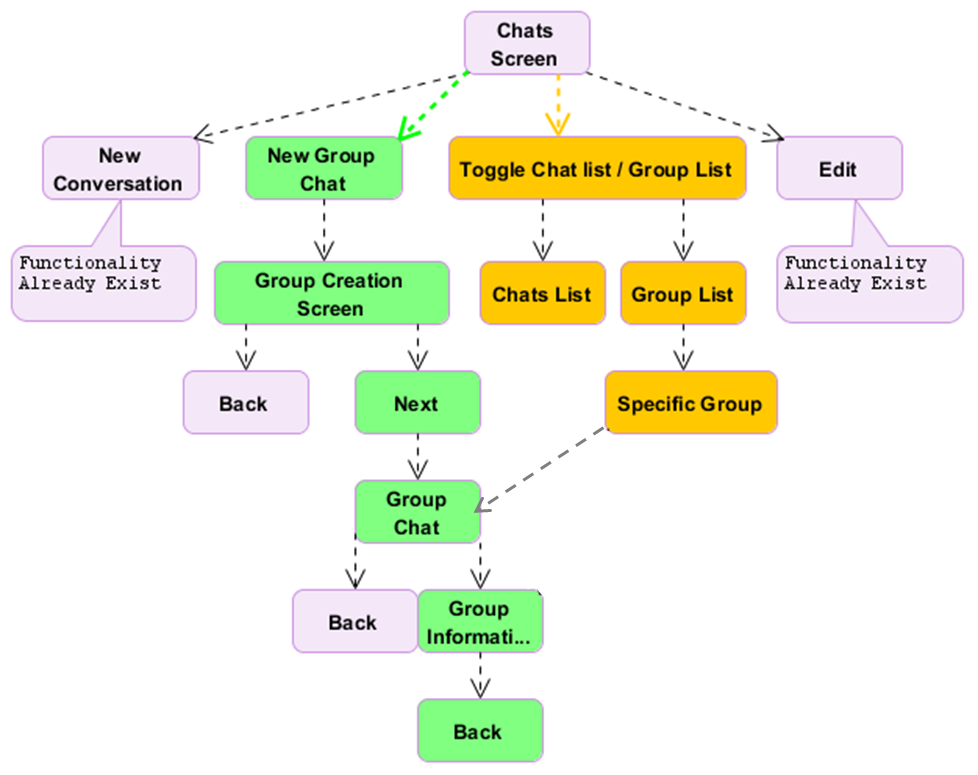
\includegraphics[width=300px]{./images/flow.png}

When on the "Chat" user interface, one will be presented with the following options on the top panel of the screen:
\begin{itemize}
\item New Conversation
\item New Group Chat
\item Edit
\end{itemize}

Looking at the diagram above, the steps to navigate through the user interface will be listed:
\textbf{Green Path}
\begin{enumerate}
\item Once logged in you will be presented with the application user interface
\item Click on the "Chat" menu item located on the bottom panel
\item Click "New Group Chat" option located on the top panel
\item You will be presented with a screen to enter neccessary information to create a new group chat
\subitem Enter a desired group name
\subitem Choose the type of encryption you wish to use
\subitem Add members to participate in the group chat - Note: at least two members must be added
\subitem Click "Next"
\item You will now be presented with the actual group chat
\item You can now proceed to "chat" in the group chat or view the group information by clicking on "Group Info" in the group chat
\subitem You can edit the information by clicking "Edit" and changing the information desired.
\end{enumerate}



\section{Troubleshooting}

\section{Appendix B}
\listoffigures

\end{document}
